\subsection{Launcher}

Le lanceur du jeu est un élément crucial, car il permet d'installer 
le jeu et de le maintenir à jour. Une première version du launcher avait 
été créée avec Avalonia, un Framework C\#. Cependant, il faisait appel à des 
librairies externes, ce qui l'alourdissait et rendait son fonctionnement instable. 
C'est pour cette raison que nous avons décidé, pour la deuxième soutenance, de nous 
tourner vers le Framework Electron, qui est parfaitement compatible avec toutes les 
plateformes car il repose sur du HTML.

\begin{figure}[hbt!]
    \centering
    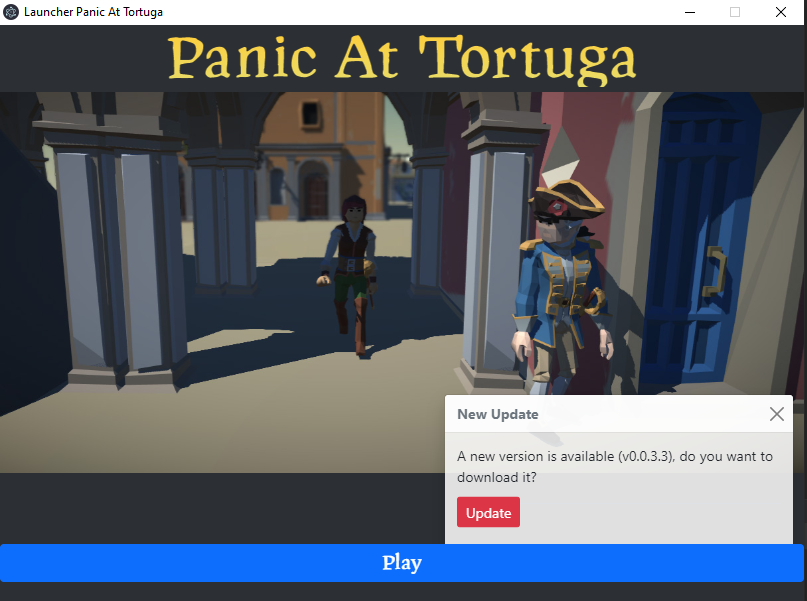
\includegraphics[scale=0.53]{launcher.png}
    \caption{Aperçu du Launcher}
\end{figure}

Le lanceur du jeu sous Electron est capable de se connecter au repo Github et de récupérer la 
dernière version du jeu afin de la comparer à la version actuelle pour proposer une éventuelle 
mise à jour. Cela permet de constamment maintenir le jeu à jour, pour éviter des conflits de versions 
ou toutes autres erreurs. Le html utilisé permet aussi de s'adapter parfaitement à toutes les formes de 
fenêtres sans problèmes d'échelles ou d'overlay.
